\section{Theory background}
This section provides the required theoretical background an GANs in general and Wasserstein GAN in particular. 
\subsection{Generative adversarial networks (GANs)}
The goal of generative adversarial networks is to produce realistic data samples by learning from a given data set $D$. This can be accomplished by learning the underlying probability distribution of the data set $P_r$.\\
\indent There are two approaches for learning $P_r$:
\begin{enumerate}
	\item To learn $P_r$ directly be defining parametrized $P_\theta$ and finding parameters $\theta$ using the \textit{maximum likelihood estimation} (MLE)
	\item To use an input noise variable $z$ with known probability density function $p_z(z)$ and define a parametrized mapping function $g_\theta: Z \rightarrow D$. Then, the density function of generated samples in denoted by $p_g(g_\theta(z))$. 
\end{enumerate}

While the first approach seems more straightforward, there are some problems with it. Maximizing the mean logarithm of the objective function $MLE(\theta)$ is equivalent to minimizing the \textit{Kullback-Leibler divergence} between two distributions $KL(P_r \lVert P_\theta)$:

\begin{align*}
	\lim_{m \to \infty} \max_{\theta} \frac{1}{m} \log MLE(\theta)
	&= \max_\theta \int_x p_r(x) \log p_\theta(x) dx \\
	&= \min_\theta - \int_x p_r(x) \log p_\theta(x) dx \\
	&= \min_\theta \int_x p_r(x) \log p_r(x) dx - \int_x p_r(x) \log p_\theta(x) dx \\
	&= \min_\theta KL(P_r \lVert P_\theta)
\end{align*}

If there is at least one data point $x \in P_r$ which has $p_\theta(x) = 0$, then KL-divergence will immediately be infinitely large. This is a common scenario in practice, because $P_\theta$ tries to find a low dimensional manifold in the space of the observed data, and there are points lying outside of this manifold. In practice, a workaround to this problem is to add noise to the model, to make sure that $P_\theta$ is defined everywhere. This however is not an ideal solution because it degrades the sample quality. \\
  
\indent Generative adversarial networks implement the latter approach with a mapping function $g_\theta$ being encoded using a neural network, called \textit{generator} $G$. Instead of the MLE generative adversarial networks use \textit{adversarial training} to find parameters for the generator. To judge the quality of the generator $G$ another network is used, \textit{discriminator}, which takes an input sample and outputs the probability that the sample comes from the real data set. The architecture of a GAN is shown in Figure~\ref{fig:gan}.\\

\begin{figure}[h]
	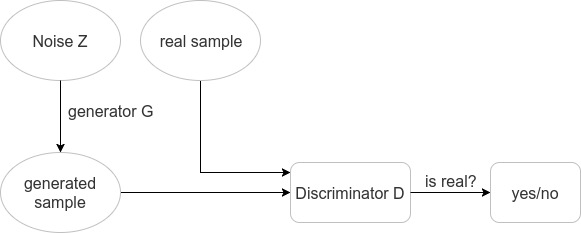
\includegraphics[width=\textwidth]{figures/gan}
	\caption{Visualization of how different parts of a GAN are connected with each other. A generator network $G$ produces samples from a noise variable $Z$. A discriminator network $D$ takes both real and generated samples and tries to distinguish between them.}
	\label{fig:gan}
\end{figure}

\indent In order to train a model one has to define two loss functions. One that shows how well a discriminator $D$ can distinguish between a real probability distribution $p_r(x)$ and its approximation computed by a generator $G$, $p_g(G(z))$. Second loss function show how well the generator can approximate the real distribution. For a standard GAN these loss functions are defined as: 
\begin{equation} \label{eq:gan_loss}
\argmin_G \argmax_D L(G,D) = \E_{x \sim p_r(x)} [\log(D(x)] + \E_{z \sim p_z(z)}[1-\log(D(G(z))]
\end{equation}
Let us analyze equation~\ref{eq:gan_loss} from the viewpoint of a discriminator. The maximum value of $L(G,D)$ is achieved when both $\E_{x \sim p_r(x)} [\log(D(x)]$ and $\E_{z \sim p_z(z)}[(1-\log(D(G(z)))]$ are equal to zero. For this to be the truth, the values inside of the  logarithms should be equal to one. This means, that the discriminator should output one for real samples and zero for generated ones. When optimizing with respect to the generator the first term of equation~\ref{eq:gan_loss} is constant. And the term $\E_{z \sim p_z(z)}[1-\log(D(G(z))]$ is equal to zero when the discriminator thinks that the samples generated by the generator are real. There is no closed form solution for~\ref{eq:gan_loss}, therefore optimization consists for applying a gradient descent optimization to the generator and to discriminator alternately.\\  

\indent A natural question that arises after looking at the adversarial training procedure is how does it relate to measuring distance between the real distribution $P_r$ and the generated one $P_G$. 

First observation is that with a generator $G$ fixed, optimal discriminator $D$ is equal to
\begin{equation}
	D^*(x) = \frac{p_r(x)}{p_r(x) + p_g(x)}
\end{equation}
Prove is trivial and can be found in the original paper~\citep{gan}.\\
Now with an optimal discriminator $D^*$ we can rewrite $L(G,D)$ as following
\begin{align*}
	L(G, D) &= \E_{x \sim p_r(x)} [\log(D^*(x)] + \E_{z \sim p_z(z)}[1-\log(D^*(G(z))] \\
	&= \E_{x \sim p_r(x)} [\log(D^*(x)] + \E_{x \sim p_g}[1-\log(D^*(x)] \\
	&= \E_{x \sim p_r(x)} \bigg[\frac{p_r(x)}{p_r(x) + p_g(x)}\bigg] + \E_{x \sim p_g}\bigg[\frac{p_g(x)}{p_r(x) + p_g(x)}\bigg] \\
	&= -\log 4 + \E_{x \sim p_r(x)} \bigg[\frac{p_r(x)}{\frac{p_r(x) + p_g(x)}{2}}\bigg] + \E_{x \sim p_g}\bigg[\frac{p_g(x)}{\frac{p_r(x) + p_g(x)}{2}}\bigg] \\
	&= -\log 4 + KL\bigg(P_r \lVert \frac{P_r + P_g}{2}\bigg) +  KL\bigg(P_g \lVert \frac{P_r + P_g}{2}\bigg) \\
	&= -\log 4 + 2 \cdot JSD(P_r \lVert P_g),
\end{align*}
where $JSD(P_r \lVert P_g)$ is the \textit{Jensen-Shannon divergence} between two distributions. Since the JS divergence is defined everywhere, this approach does not suffer from the problems described for MLE.

\indent We have shown that assuming that a discriminator is always trained to optimality, objective function defined in equation~\ref{eq:gan_loss} can be interpreted as a Jensen-Shannon divergence between the real distribution $P_r$ and the one approximated by a generator $P_g$. 

\subsection{Wasserstein GANs (WGANs)}
Wasserstein GANs were introduced in January 2017~\citep{wgan}. Authors argue that Jensen-Shannon divergence, used in original GANs to calculate the distance between generated and original probability distributions, has some problems and proposed a new objective function based on the \textit{Earth-Mover} (EM)  distance. This distance should improve stability of the training process and provide a distance measure that corresponds to the perceived sample quality. 
	The Earth-Mover distance between two distributions is defined by
\begin{equation}
	W(P_g, P_r) =  \inf_{\gamma \in \prod (P_r, P_g)}  \E_{(x,y) \sim \gamma} [ \lVert x - y \lVert ],
\end{equation}
where $\prod (P_r, P_g)$ is a set of all joint distributions $\gamma(x,y)$ whose marginal distributions are $P_r$ and $P_g$ respectively. To understand the idea behind the EM distance we can imagine that probability distributions assign a mass to each point $x$ and we want to turn distribution $P_r$ into $P_g$ by moving this mass around. Furthermore, moving a mass $m$ by a distance $d$ would cost us $m \cdot d$ effort. In this imaginary scenario the EM distance will give us the minimal effort we would have to spend. Why is this true? 
\begin{itemize}
	\item Each $\gamma(x, y)$ can represent the amount of mass transported between points $x$ and $y$, then in our scenario $\gamma$ will represent a "transport plan" for transitioning from $P_r$ to $P_g$.
	\item For $\gamma$ to be a valid strategy it has to satisfy several conditions:
		\subitem Amount of mass leaving point $x$ is calculated by $\int_y \gamma(x, y) dy$ and should be equal to $p_r(x)$, the amount of mass originally located at $x$
		\subitem In the same way, the amount of mass entering $y$ is calculated by $\int_x \gamma(x, y) dx$ and should be equal to $p_g(y)$, the amount of mass located at $y$ at the end.
	\item These conditions mean that marginal distributions of $\gamma(x, y)$ should equal to $P_r$ and $P_g$ respectively. 
	\item The amount of effort required to execute the transporting plan $\gamma$ is 
	\begin{equation}
	\int_x \int_y \gamma(x,y) \lVert x - y \lVert dx dy = \E_{(x,y) ~\sim \gamma} [ \lVert x - y \lVert ]
	\end{equation}
	\item Infinum over this effort gives the EM distance. 
\end{itemize}

One property that is expected from an objective function is that it is continuous and differentiable in its whole domain. And this is exactly where EM distance outperforms the Jensen-Shannon divergence, which is illustrated in the original paper a nice example. 

Consider a uniform random variable $Z \in [0, 1]$ and a distribution $P_r = (0, Z) \in \mathbb{R}^2$. Let $g_\theta(z) = (\theta, z)$ be the mapping function with a single parameter $\theta$. Now we can compute the Jensen-Shannon divergence and the EM distance between $P_r$ and $P_g$. 
To compute the Jensen-Shannon divergence let us first compute $KL(P_r \lVert M)$ where $M = \frac{1}{2}P_r + \frac{1}{2}P_g$:
\begin{equation}
	KL(P_r \lVert M) = \int_{x,y} p_r(x,y) \log \frac{p_r(x,y)}{m(x,y)} dxdy = \log2,
\end{equation}
because $m(x,y) = \frac{1}{2} p_r(x,y)$ everywhere except for points with $x=0$ or $x=\theta$. The same is true for $KL(P_r \lVert M)$ and therefore:
\begin{align*}
 JSD(P_r \lVert P_g) &= \frac{1}{2}KL(P_r \lVert M) + \frac{1}{2}KL(P_g\lVert M) \\ 
 	&= \begin{cases}
 		\log2, & \text{if } \theta \neq 0 \\
 		0, & \text{if } \theta = 0
 	\end{cases}.
\end{align*}  
On the other hand, if we recall the example explaining the intuition behind the ME distance, we can see that to transport all the mass from $P_r$ to $P_\theta$ we need to transport each mass point by distance $\theta$, therefore
\begin{equation}
	M(P_r, P_g) = \int_{(0,z)} |\theta| \cdot p_r(0,z)dz = |\theta|
\end{equation}

Already from this example we can see that there are cases where the EM distance is continuous whilst JS divergence not. Authors have shown that if a mapping function $g_\theta(x)$ is itself continuous, so that is the EM distance $M(P_r, P_g)$. Moreover, if $g_\theta(x)$ fulfills certain criteria, EM distance will be differentiable almost in the whole domain. At the same time, both statements are false for the JS divergence~\citep{wgan}. The criteria for the function $g_\theta(x)$ to be fulfilled are:
\begin{enumerate}
	\item The function $g_\theta$ is \textit{locally Lipschitz continuous}. \\
	A real-valued function $g_\theta$ is called Lipschitz continuous if there exists a constant $K$, called a \textit{Lipschitz constant}, such that for all $x_1$ and $x_2$:
	\begin{equation}
		\lVert g_\theta(x_1) - g_\theta(x_2) \lVert \leq K\lVert x_1 - x_2 \lVert
	\end{equation}  
	Local Lipschitz continuity means that for each point $x$ there exists a neighborhood $U$ where $g_\theta$ is Lipschitz continuous. \\
	In other words, Lipschitz continuity restricts how fast a function can change, because for every two points of the function the absolute angle of a line connecting their function values is restricted by a constant $K$. 
	\item The function $g_\theta$ satisfies \textit{regularity assumption 1}. \\
	Let $K(\theta, z)$ denote the local Lipschitz constant at point $(\theta, z)$ of a locally Lipschitz continuous function $g_\theta(z)$. Then, $g_\theta$ satisfies the regularity assumption 1 if the expected value of $K(\theta, z)$ is upper-bounded:
	\begin{equation}
		\E_z[K(\theta, z)] < +\infty
	\end{equation}
\end{enumerate} 
While these assumptions are tedious to prove manually for each mapping function $g_\theta$, authors have shown that all feed-forward neural networks with pointwise or rectified nonlinearities satisfy both these requirements and therefore when using such networks to encode a  generator of a GAN, the EM distance will be continuous and differentiable almost everywhere.  

To utilize the properties of the EM distance we should be able to compute it efficiently. Unfortunately, computing it exactly is not feasible, therefore we have to approximate. 
Firstly, we can use the Kantorovich-Rubinstein duality to rewrite $W(P_r, P_\theta)$ as following
\begin{equation}
	W(P_r, P_\theta) = \sup_{\lVert f \lVert_L \leq 1} \E_{x \sim P_r}[f(x)] - E_{x \sim P_\theta} [f(x)],	
\end{equation}
where ${\lVert f \lVert_L \leq 1}$ denotes the set of all functions that are Lipschitz continuous with Lipschitz constant equal $1$, or also called \textit{1-Lipschitz} functions. If we replace this set with ${\lVert f \lVert_L \leq K}$ we will receive the upper bound for $K \cdot W(P_r, P_\theta)$ instead, which is still intractable to compute but easier to approximate. As already discussed, a discriminator $D$  encoded using a neural network with parameters $w$ is a $K$-Lipschitz function. Therefore
\begin{align*}
\max_w \E_{x \sim P_r}[D(x)] - E_{x \sim P_\theta} [D(x)] &\leq \sup_{\lVert D \lVert_L \leq K} \E_{x \sim P_r}[D(x)] - E_{x \sim P_\theta} [D(x)] \\
 &= K \cdot W(P_r, P_\theta)
\end{align*}
Note, that supremum may not be achieved, if there is a $K$-Lipschitz function that can not be encoded with parameters $\theta$ or if the supremum is achieved for some $k$-Lipschitz function with $k < K$.

One thing that is remained to do is to ensure that $K$ remains constant during the training process. One obvious way to do that is to restrict the space $S$ of possible function encoded by $D$, then the set of possible Lipschitz constants will be upper-bounded. We enforce discriminators to lie in $S$ by defining an upper and a lower bound for all weights of a discriminant, which will remain unchanged throughout the training process.
 
To train the discriminator we have to compute the gradients of $W(P_r, P_\theta)$ with respect to $w$. In the same way, updates for Generator $G$ are obtained by computing the gradients with respect to $\theta$ 
\begin{align*}
\nabla_\theta W(P_r, P_\theta) &= \nabla_\theta(\E_{x \sim P_r}[D(x)] - E_{z \sim Z} [D(G(z))]) \\
&= - \E_{z \sim Z} [\nabla_\theta D(G(z))]
\end{align*}

The training process therefore consists of the following steps:
\begin{enumerate}
	\item For a fixed generator train the discriminator to convergence in order to obtain the approximation of $W(P_r, P_\theta)$.s
	\item With an optimal discriminator update the generator by computing the gradient $- \E_{z \sim Z} [\nabla_\theta D(G(z))]$
	\item Enforce the discriminator $D$ to remain $K$-Lipschitz by clipping its to values $[-c, c]$, where $c$ remains constant during the training process. 
\end{enumerate}

Apart from the fact that the Wasserstein GAN allows more stable training, its loss function corresponds to the image quality. This is illustrated in figures~\ref{fig:losses} and~\ref{fig:samples_evolution}.

\begin{figure}
  \begin{subfigure}[b]{0.5\textwidth}
    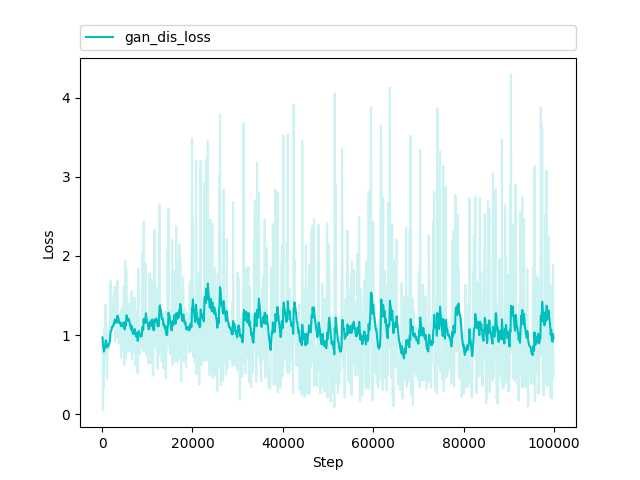
\includegraphics[width=\textwidth]{figures/gan_dis_loss}
    \caption{GAN discriminator loss}
    \label{fig:gan_dis_loss}
  \end{subfigure}
  \hfill
  \begin{subfigure}[b]{0.5\textwidth}
    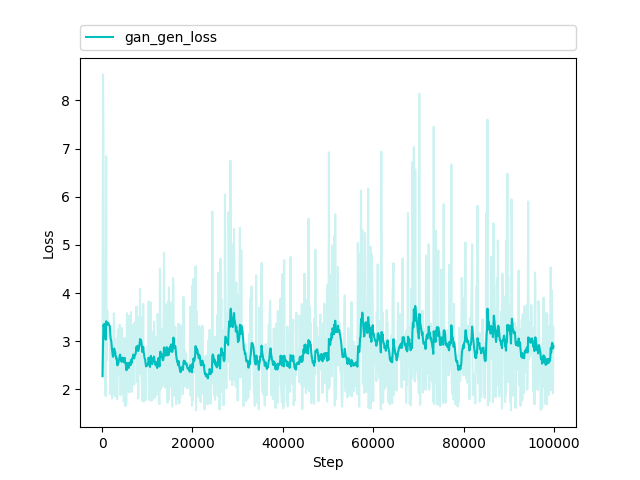
\includegraphics[width=\textwidth]{figures/gan_gen_loss}
    \caption{GAN generator loss}
    \label{fig:gan_gen_loss}
  \end{subfigure}
  \begin{subfigure}[b]{0.5\textwidth}
    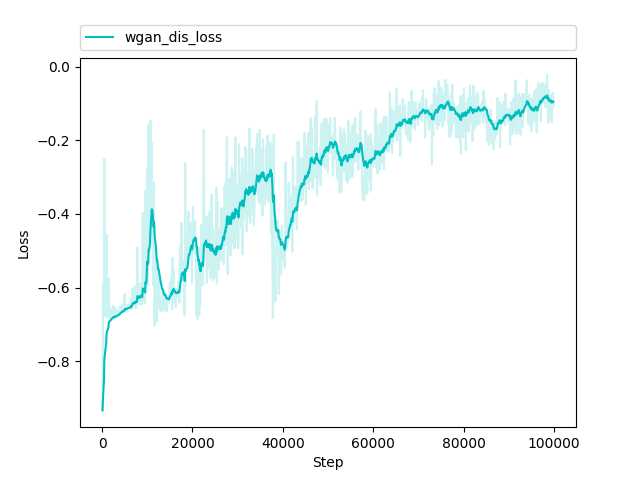
\includegraphics[width=\textwidth]{figures/wgan_dis_loss}
    \caption{Wasserstein GAN discriminator loss}
    \label{fig:wgan_dis_loss}
  \end{subfigure}
  \hfill
  \begin{subfigure}[b]{0.5\textwidth}
    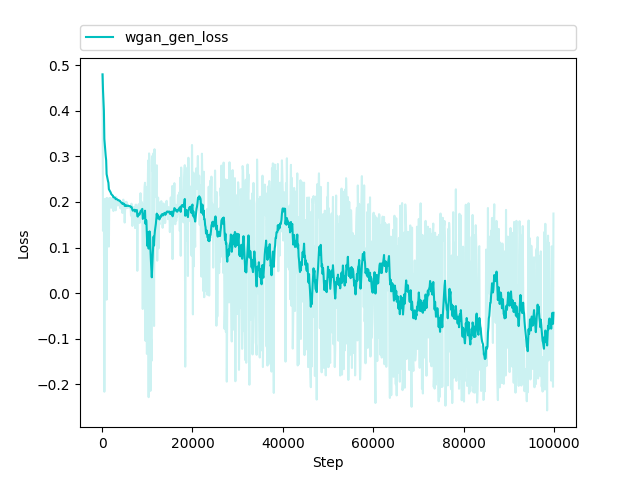
\includegraphics[width=\textwidth]{figures/wgan_gen_loss}
    \caption{Wasserstein GAN generator loss}
    \label{fig:wgan_gen_loss}
  \end{subfigure}
  
  \caption{Figures illustrating that WGAN has a correlation between the number of training steps and the values of its objective functions. On the other hand the objective functions of a GAN remain in the same interval although the quality of the samples increases.}
  \label{fig:losses}
\end{figure}
\begin{figure}
  \begin{subfigure}[b]{\textwidth}
    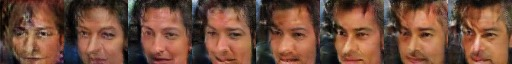
\includegraphics[width=\textwidth]{figures/gan_progress}
    \caption{Evolution of GAN generated samples quality}
    \label{fig:gan_evolution}
  \end{subfigure}
  \begin{subfigure}[b]{\textwidth}
    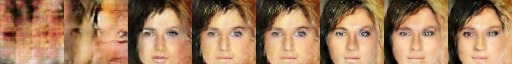
\includegraphics[width=\textwidth]{figures/wgan_progress}
    \caption{Evolution of Wasserstein GAN generated samples quality}
    \label{fig:gan_evolution}
  \end{subfigure}
  \caption{Samples generated after different number of training steps. Each sample is generated from the same noise variable.}
  \label{fig:samples_evolution}
\end{figure}


\subsection{Improved WGANs}





